\documentclass[11pt,a4paper]{article}
\usepackage[margin=2.5cm]{geometry}
\usepackage{tikz}
\usetikzlibrary{arrows.meta,shapes.geometric,fit,positioning,calc,shadows}
\usepackage{listings}
\usepackage{booktabs}
\usepackage{xcolor}
\usepackage{hyperref}
\usepackage[T1]{fontenc}
\usepackage{microtype}
% enumitem not available in basic installation; using standard list environments
\usepackage{fancyhdr}
\usepackage{tabularx}
\usepackage{multicol}
\usepackage{lmodern}

%% ── Colour palette ──────────────────────────────────────────────────────────
\definecolor{primary}{HTML}{4F46E5}    % indigo
\definecolor{secondary}{HTML}{0EA5E9}  % sky
\definecolor{success}{HTML}{10B981}    % green
\definecolor{warning}{HTML}{F59E0B}    % amber
\definecolor{danger}{HTML}{EF4444}     % red
\definecolor{codebg}{HTML}{F8F9FA}
\definecolor{codefg}{HTML}{1E293B}

%% ── Code listing style ──────────────────────────────────────────────────────
\lstdefinestyle{pythonstyle}{
  language=Python,
  backgroundcolor=\color{codebg},
  basicstyle=\ttfamily\small\color{codefg},
  keywordstyle=\color{primary}\bfseries,
  stringstyle=\color{success},
  commentstyle=\color{gray}\itshape,
  breaklines=true,
  breakatwhitespace=true,
  frame=single,
  framesep=4pt,
  rulecolor=\color{primary!30},
  numbers=left,
  numberstyle=\tiny\color{gray},
  xleftmargin=1.5em,
  showstringspaces=false,
  tabsize=4,
}
\lstset{style=pythonstyle}

%% ── Header / footer ─────────────────────────────────────────────────────────
\pagestyle{fancy}
\fancyhf{}
\fancyhead[L]{\small\color{gray}llm-guard-kit v0.17.0}
\fancyhead[R]{\small\color{gray}Architecture \& API Reference}
\fancyfoot[C]{\small\thepage}
\renewcommand{\headrulewidth}{0.4pt}

%% ── Hyperref ─────────────────────────────────────────────────────────────────
\hypersetup{
  colorlinks=true,
  linkcolor=primary,
  urlcolor=secondary,
  citecolor=success,
  pdftitle={llm-guard-kit v0.17.0 Architecture},
  pdfauthor={llm-guard-kit},
}

% ─────────────────────────────────────────────────────────────────────────────
\begin{document}

%% ── Cover page ───────────────────────────────────────────────────────────────
\begin{titlepage}
\thispagestyle{empty}
\begin{tikzpicture}[remember picture, overlay]
  \fill[primary] (current page.north west) rectangle
    ([yshift=-7cm]current page.north east);
\end{tikzpicture}

\vspace*{2.5cm}

{\color{white}\Huge\bfseries llm-guard-kit}

\vspace{0.5cm}
{\color{white!80}\Large v0.17.0 Architecture, Usage Guide \& API Reference}

\vspace{1.2cm}
\noindent\colorbox{warning!90}{%
  \parbox{0.9\textwidth}{\color{white}\centering\large
    Real-time confidence scoring for LLM agents ---
    AUROC 0.817 at \$0 inference cost
  }%
}

\vspace{3.5cm}

\begin{tabular}{ll}
  \textbf{Date:}   & \today \\[4pt]
  \textbf{PyPI:}   & \url{https://pypi.org/project/llm-guard-kit/} \\[4pt]
  \textbf{GitHub:} & \url{https://github.com/Avighan/llm-guard-kit} \\[4pt]
  \textbf{Version:} & 0.17.0 \\
\end{tabular}

\vfill

{\small\color{gray}
  llm-guard-kit is an open-source library for real-time reliability
  monitoring of multi-step LLM agents. It detects failures, assigns
  confidence tiers, and routes to recovery adapters --- all with
  validated AUROC scores reported on held-out evaluation sets.
}
\end{titlepage}

\newpage
\tableofcontents
\newpage

% ─────────────────────────────────────────────────────────────────────────────
\section{Executive Summary}
% ─────────────────────────────────────────────────────────────────────────────

\subsection*{Problem}

Multi-step LLM agents using ReAct-style reasoning (think $\to$ search $\to$ observe $\to$
repeat) fail silently. When a search returns empty results, the agent loops, guesses,
or confidently produces a wrong answer. There is no built-in mechanism to detect
these failures before they propagate to users or downstream agents.

\subsection*{Solution}

\textbf{llm-guard-kit} monitors every reasoning chain in real time. It computes a
\texttt{risk\_score} $\in [0,1]$ by combining:
\begin{itemize}
  \item \textbf{SC\_OLD behavioral signals} (\$0, 19\,ms): 12 structural features
        extracted from the chain (loop rate, empty-observation rate, repeated-query
        rate, step count, etc.) fed into a fitted logistic-regression ensemble.
  \item \textbf{MiniJudge} (\$0): a LogReg distilled from Sonnet judge decisions,
        shipped as a pre-trained \texttt{.pkl} inside the package (AUROC 0.747).
  \item \textbf{P(True) via Haiku} ($\sim$\$0.0003): prompts Haiku to rate answer
        correctness on a 1-5 scale, domain-agnostic.
  \item \textbf{Sonnet judge} ($\sim$\$0.007): full-chain GOOD/BORDERLINE/POOR
        verdict for highest cross-domain precision.
\end{itemize}

\subsection*{Key Results}

\begin{table}[h]
\centering
\begin{tabular}{lrrr}
\toprule
\textbf{Signal} & \textbf{Within-Domain AUROC} & \textbf{Cross-Domain AUROC} & \textbf{Cost/Chain} \\
\midrule
MiniJudge (behavioral LogReg) & $0.747 \pm 0.10$ & --- & \$0 \\
SC\_OLD behavioral ensemble   & 0.817            & 0.703 (2Wiki) / 0.659 (TV) & \$0 \\
SC\_OLD + P(True) (Haiku)     & ---              & 0.74 & $\sim$\$0.0003 \\
SC\_OLD + Sonnet judge        & 0.777            & 0.741 & $\sim$\$0.007 \\
Alert precision @ FPR $\leq$ 10\% & 0.908       & ---  & --- \\
\bottomrule
\end{tabular}
\caption{Validated performance on held-out evaluation sets. Within-domain = HotpotQA
(200 chains). Cross-domain = TriviaQA n=1000, 2WikiMultiHop n=200.}
\end{table}

% ─────────────────────────────────────────────────────────────────────────────
\section{System Architecture}
% ─────────────────────────────────────────────────────────────────────────────

The figure below shows the layered architecture of \texttt{llm-guard-kit}.

\begin{center}
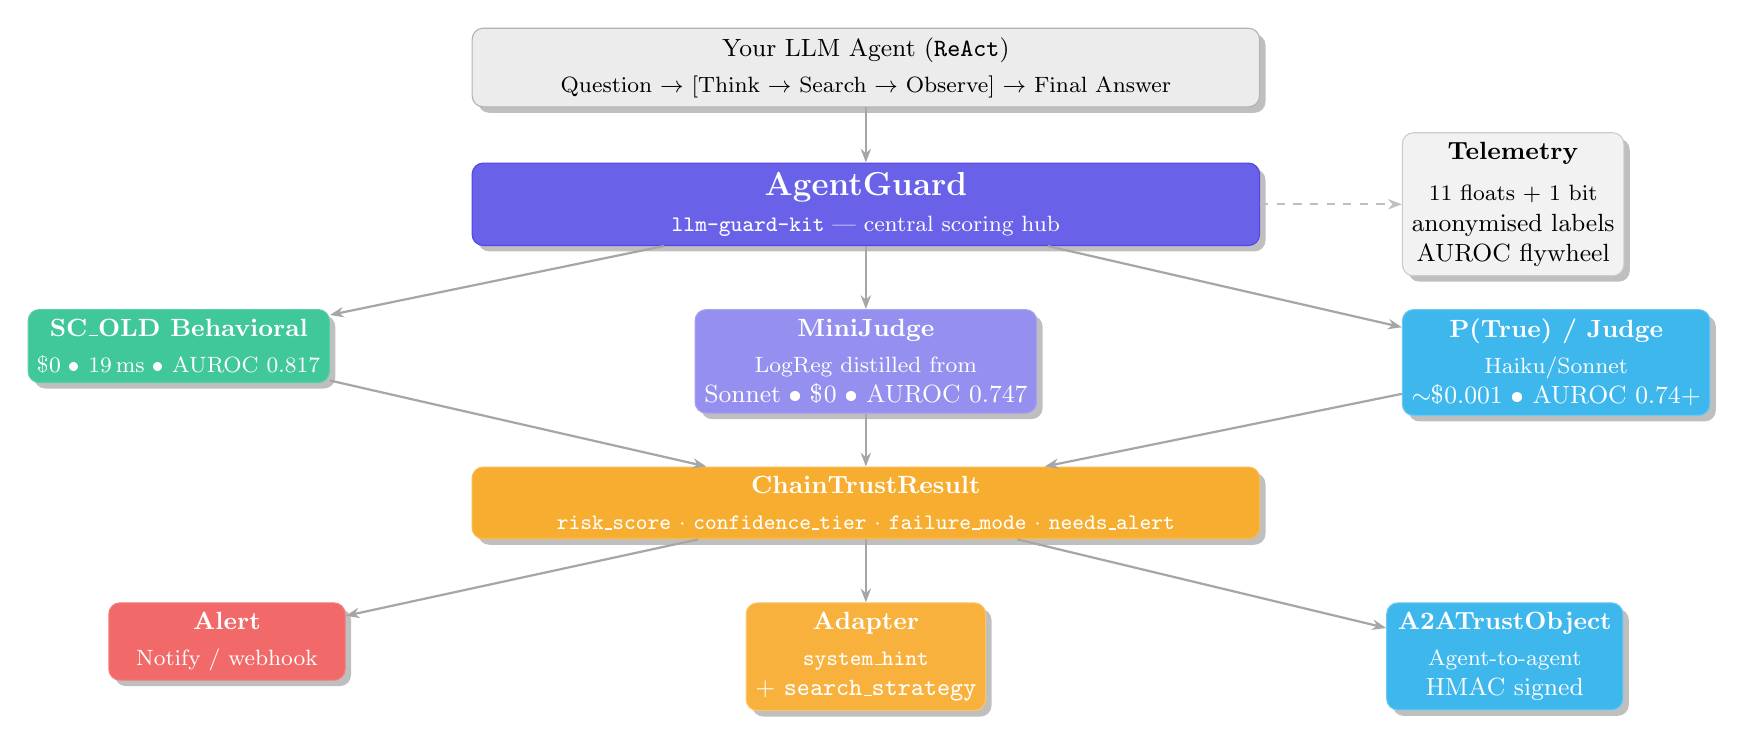
\begin{tikzpicture}[
  every node/.style={font=\small},
  box/.style={draw, rounded corners=4pt, minimum width=3.2cm, minimum height=0.8cm,
              align=center, drop shadow},
  layer1/.style={box, fill=gray!15, draw=gray!60},
  layer2/.style={box, fill=primary!85, text=white, draw=primary},
  layer3L/.style={box, fill=success!80, text=white, draw=success!70, minimum width=3.5cm},
  layer3C/.style={box, fill=primary!60, text=white, draw=primary!50, minimum width=3.5cm},
  layer3R/.style={box, fill=secondary!80, text=white, draw=secondary!60, minimum width=3.5cm},
  layer4/.style={box, fill=warning!85, text=white, draw=warning!70, minimum width=10cm},
  out_alert/.style={box, fill=danger!80, text=white, draw=danger!70, minimum width=3cm},
  out_adapt/.style={box, fill=warning!80, text=white, draw=warning!60, minimum width=3cm},
  out_trust/.style={box, fill=secondary!80, text=white, draw=secondary!60, minimum width=3cm},
  tel/.style={box, fill=gray!10, draw=gray!40, minimum width=2.8cm, minimum height=1.4cm},
  arr/.style={-{Stealth[length=5pt]}, thick, color=gray!70},
]

%% Layer 1: Your Agent
\node[layer1, minimum width=10cm] (agent)
  {Your LLM Agent (\texttt{ReAct})\\[2pt]
   \footnotesize Question $\to$ [Think $\to$ Search $\to$ Observe] $\to$ Final Answer};

%% Layer 2: AgentGuard
\node[layer2, minimum width=10cm, below=0.7cm of agent] (guard)
  {\large\textbf{AgentGuard}\\[2pt]
   \footnotesize \texttt{llm-guard-kit} — central scoring hub};

%% Layer 3: Three signal columns
\node[layer3L, below left=0.8cm and 1.8cm of guard] (beh)
  {\textbf{SC\_OLD Behavioral}\\[2pt]\footnotesize\$0\ \textbullet\ 19\,ms\ \textbullet\ AUROC 0.817};

\node[layer3C, below=0.8cm of guard] (mini)
  {\textbf{MiniJudge}\\[2pt]\footnotesize LogReg distilled from\\Sonnet \textbullet\ \$0 \textbullet\ AUROC 0.747};

\node[layer3R, below right=0.8cm and 1.8cm of guard] (ptrue)
  {\textbf{P(True) / Judge}\\[2pt]\footnotesize Haiku/Sonnet\\$\sim$\$0.001\ \textbullet\ AUROC 0.74+};

%% Layer 4: ChainTrustResult
\node[layer4, below=2.8cm of guard] (result)
  {\textbf{ChainTrustResult}\\[2pt]
   \footnotesize \texttt{risk\_score}\ $\cdot$\ \texttt{confidence\_tier}\ $\cdot$\ \texttt{failure\_mode}\ $\cdot$\ \texttt{needs\_alert}};

%% Layer 5: Three outputs
\node[out_alert, below left=0.8cm and 1.6cm of result] (alert)
  {\textbf{Alert}\\[2pt]\footnotesize Notify / webhook};

\node[out_adapt, below=0.8cm of result] (adapt)
  {\textbf{Adapter}\\[2pt]\footnotesize \texttt{system\_hint}\\+ \texttt{search\_strategy}};

\node[out_trust, below right=0.8cm and 1.6cm of result] (trust)
  {\textbf{A2ATrustObject}\\[2pt]\footnotesize Agent-to-agent\\HMAC signed};

%% Telemetry side-box
\node[tel, right=1.8cm of guard] (tel)
  {\textbf{Telemetry}\\[4pt]
   \footnotesize 11 floats + 1 bit\\anonymised labels\\AUROC flywheel};

%% Arrows
\draw[arr] (agent) -- (guard);
\draw[arr] (guard) -- (beh);
\draw[arr] (guard) -- (mini);
\draw[arr] (guard) -- (ptrue);
\draw[arr] (beh)   -- (result);
\draw[arr] (mini)  -- (result);
\draw[arr] (ptrue) -- (result);
\draw[arr] (result) -- (alert);
\draw[arr] (result) -- (adapt);
\draw[arr] (result) -- (trust);
\draw[arr, dashed, color=gray!50] (guard) -- (tel);

\end{tikzpicture}
\end{center}

% ─────────────────────────────────────────────────────────────────────────────
\section{Component Reference}
% ─────────────────────────────────────────────────────────────────────────────

\subsection{MiniJudge --- \$0 Local Judge}

\textbf{What it is:} A pre-trained \texttt{sklearn} pipeline
(StandardScaler + LogisticRegression on 11 SC\_OLD features) distilled from
Sonnet judge verdicts. Shipped as a \texttt{.pkl} inside the package.

\textbf{When to use:} Drop-in replacement for Haiku/Sonnet when API access
is unavailable or cost is constrained. Ideal for CI/CD pipelines and batch
evaluation.

\textbf{Performance:} AUROC $0.747 \pm 0.10$ (5-fold CV, HotpotQA 200 chains,
exp159). Cost: \$0.000/chain.

\begin{lstlisting}
from llm_guard import MiniJudge

judge = MiniJudge()          # auto-loads bundled pkl
risk  = judge.score(question, steps, final_answer)  # -> float [0,1]

# Score using alias (drop-in with AgentGuard)
risk  = judge.score_chain(question, steps, final_answer)

# Retrain on your own labeled data
judge.fit(labeled_chains)    # each chain needs "correct" bool field
\end{lstlisting}

% ─────────────────────────────────────────────────────────────────────────────
\subsection{AgentGuard (Behavioral) --- Production Baseline}

\textbf{What it is:} Behavioral SC\_OLD scoring using 12 structural features
extracted from the ReAct chain. Fitted logistic-regression ensemble with
no API dependency.

\textbf{When to use:} Default choice for production. \$0 cost, 19\,ms p50 latency.
AUROC 0.817 within HotpotQA, 0.659--0.703 cross-domain.

\textbf{Performance:} AUROC 0.817 within-domain; alert precision 0.908 at
FPR $\leq 10\%$ (exp92 conformal calibration).

\begin{lstlisting}
from llm_guard import AgentGuard

guard  = AgentGuard()   # no API key needed
result = guard.score_chain(question, steps, final_answer)

print(result.risk_score)        # float [0,1]
print(result.confidence_tier)   # "HIGH" / "MEDIUM" / "LOW"
print(result.needs_alert)       # True when risk >= 0.70
print(result.failure_mode)      # "retrieval_fail" / None / ...
print(result.behavioral_score)  # SC_OLD score before any blending
\end{lstlisting}

% ─────────────────────────────────────────────────────────────────────────────
\subsection{AgentGuard + P(True) --- Cross-Domain Scoring}

\textbf{What it is:} Behavioral SC\_OLD blended with a P(True) signal from
Haiku. P(True) prompts the model to rate answer correctness 1--5, providing
a domain-agnostic uncertainty signal.

\textbf{When to use:} Cross-domain deployment where the target domain differs
from the training distribution. Adds $\sim$\$0.0003/chain.

\textbf{Performance:} AUROC 0.78 cross-domain (best ensemble, exp120).

\begin{lstlisting}
from llm_guard import AgentGuard

guard  = AgentGuard(api_key="sk-ant-...")
result = guard.score_with_ptrue(question, steps, final_answer,
                                ptrue_weight=0.9)

# Or use the adaptive bandit to tune ptrue_weight automatically
guard.enable_ptrue_bandit()
result = guard.score_with_ptrue(question, steps, final_answer)
\end{lstlisting}

% ─────────────────────────────────────────────────────────────────────────────
\subsection{AgentGuard + Sonnet Judge --- Highest Precision}

\textbf{What it is:} Full J5 ensemble: SC\_OLD $\times 1$ + Sonnet judge
$\times 3$. The Sonnet judge produces GOOD/BORDERLINE/POOR chain-level verdicts.

\textbf{When to use:} Compliance-sensitive pipelines, high-stakes answers,
or when precision matters more than cost.

\textbf{Performance:} AUROC 0.777 within-domain, 0.741 cross-domain (exp89).

\begin{lstlisting}
from llm_guard import AgentGuard

guard  = AgentGuard(api_key="sk-ant-...", use_judge=True)
result = guard.score_chain(question, steps, final_answer)

print(result.judge_label)   # "GOOD" / "BORDERLINE" / "POOR"
print(result.risk_score)    # J5 = SC_OLD*1 + judge*3 (normalised)
\end{lstlisting}

% ─────────────────────────────────────────────────────────────────────────────
\subsection{stream\_guard --- Mid-Chain Abort}

\textbf{What it is:} Real-time abort decision evaluated at step~2 of the
agent loop. Combines SC\_OLD prefix scores with an optional Haiku mid-chain
judge call.

\textbf{When to use:} Long-running chains where early abort saves 3--5 LLM
calls. Particularly effective when empty observations appear at step~1--2.

\textbf{Performance:} Two-stage OR strategy achieves Recall 0.416, Precision
0.740 (vs J5-only: Recall 0.595, Precision 0.908). Use when recall matters.

\begin{lstlisting}
from llm_guard import AgentGuard

guard = AgentGuard()    # or AgentGuard(api_key=...) for Haiku judge

# Call after step 2 completes
sg = guard.stream_guard(question, steps_so_far, abort_threshold=0.65)

if sg.abort:
    print(f"Abort at step {sg.step_index}: risk={sg.risk_at_step:.3f}")
    # sg.rewritten_queries contains 3 diverse reformulations (if api_key set)
    next_query = sg.rewritten_queries[0] if sg.rewritten_queries else question
\end{lstlisting}

% ─────────────────────────────────────────────────────────────────────────────
\subsection{A2ATrustObject --- Multi-Agent Trust}

\textbf{What it is:} Structured confidence envelope passed between agents.
HMAC-SHA256 signed over 8 canonical fields (exp114). Google A2A compatible.

\textbf{When to use:} Multi-agent orchestration. Agent A emits a trust object;
Agent B conditions its strategy on the confidence tier and failure mode.

\textbf{Performance:} Round-trip pass 200/200 (100\%); tamper detection
200/200 (100\%); sign latency 0.034\,ms; wire size 458--539 bytes.

\begin{lstlisting}
from llm_guard import AgentGuard, A2ATrustObject

guard = AgentGuard()
trust = guard.generate_trust_object(question, steps, final_answer)

# Agent A: sign and transmit
trust.sign("fleet-secret-2026")
payload = trust.to_dict()   # JSON-serialisable dict

# Agent B: deserialise and verify
trust = A2ATrustObject.from_dict(payload)
assert trust.verify("fleet-secret-2026")  # raises if tampered

if trust.should_rewrite:
    # Use QueryRewriter before running Agent B
    pass
\end{lstlisting}

% ─────────────────────────────────────────────────────────────────────────────
\subsection{QuickCalibrator --- Domain Calibration}

\textbf{What it is:} One-call domain-adaptive isotonic calibration. Wraps
\texttt{calibrate\_isotonic()} into a 20-chain setup flow.

\textbf{When to use:} Cross-domain deployment where default thresholds give
too many false positives or misses. Needs 20+ labeled chains from the target
domain.

\textbf{Performance:} Isotonic calibration improves threshold precision
without changing AUROC (monotone transform). Particularly effective for
domains with different base rates of failure.

\begin{lstlisting}
from llm_guard import QuickCalibrator

cal = QuickCalibrator(min_chains=20)
cal.fit(labeled_chains, domain="my_customer_support_bot")
# labeled_chains: each dict has "question", "steps",
#                 "final_answer", "correct" (bool)

risk = cal.score(question, steps, final_answer)
# Returns calibrated risk in [0,1]
\end{lstlisting}

% ─────────────────────────────────────────────────────────────────────────────
\subsection{Platform Integrations}

\texttt{llm-guard-kit} ships 2-line drop-in callbacks for major frameworks:

\begin{lstlisting}
# LangChain
from llm_guard import AgentGuardCallback
from langchain.agents import AgentExecutor

agent = AgentExecutor(agent=..., tools=...,
                      callbacks=[AgentGuardCallback(api_key="sk-ant-...")])

# LlamaIndex
from llm_guard import AgentGuardEventHandler
from llama_index.core import Settings
Settings.callback_manager.add_handler(AgentGuardEventHandler())

# CrewAI
from llm_guard import AgentGuardCrewCallback
crew = Crew(agents=[...], tasks=[...],
            callbacks=[AgentGuardCrewCallback()])
\end{lstlisting}

% ─────────────────────────────────────────────────────────────────────────────
\section{Decision Guide}
% ─────────────────────────────────────────────────────────────────────────────

Use the flowchart below to select the right configuration for your use case.

\begin{center}
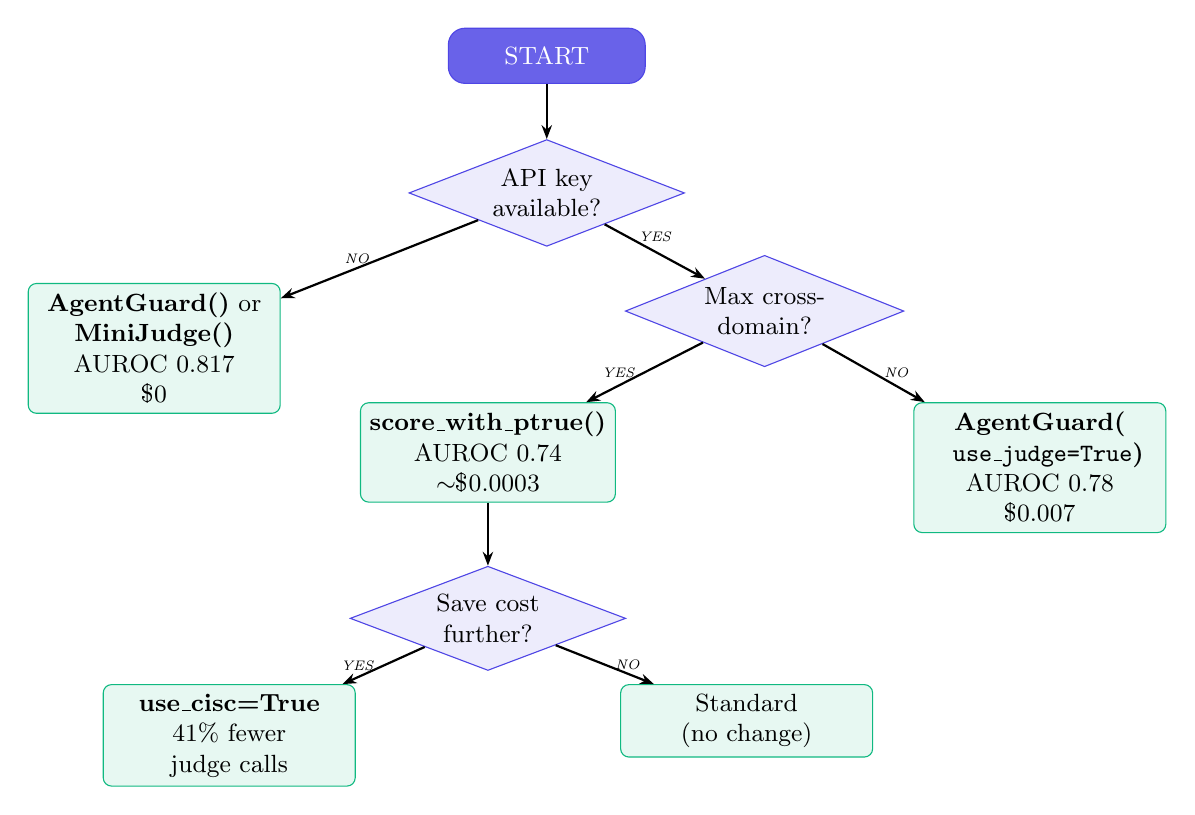
\begin{tikzpicture}[
  every node/.style={font=\small},
  decision/.style={diamond, draw=primary, fill=primary!10, aspect=2.5,
                   minimum width=3.5cm, align=center, inner sep=2pt},
  action/.style={rectangle, draw=success, fill=success!10,
                 rounded corners=3pt, minimum width=3.2cm,
                 minimum height=0.8cm, align=center},
  start/.style={rectangle, draw=primary, fill=primary!85, text=white,
                rounded corners=6pt, minimum width=2.5cm,
                minimum height=0.7cm, align=center},
  arr/.style={-{Stealth[length=5pt]}, thick},
  label/.style={font=\tiny\itshape, midway},
]

\node[start] (S) {START};

\node[decision, below=0.7cm of S] (D1)
  {API key\\available?};

\node[action, below left=0.8cm and 2.5cm of D1] (A_noapikey)
  {\textbf{AgentGuard()} or\\\textbf{MiniJudge()}\\AUROC 0.817\\\$0};

\node[decision, below right=0.8cm and 1cm of D1] (D2)
  {Max cross-\\domain?};

\node[action, below left=0.8cm and 1cm of D2] (A_ptrue)
  {\textbf{score\_with\_ptrue()}\\AUROC 0.74\\$\sim$\$0.0003};

\node[action, below right=0.8cm and 1cm of D2] (A_judge)
  {\textbf{AgentGuard(}\\\ \ \texttt{use\_judge=True}\textbf{)}\\AUROC 0.78\\\$0.007};

\node[decision, below=0.8cm of A_ptrue] (D3)
  {Save cost\\further?};

\node[action, below left=0.5cm and 0.8cm of D3] (A_cisc)
  {\textbf{use\_cisc=True}\\41\% fewer\\judge calls};

\node[action, below right=0.5cm and 0.8cm of D3] (A_std)
  {Standard\\(no change)};

\draw[arr] (S) -- (D1);
\draw[arr] (D1) -- node[label, left]{NO} (A_noapikey);
\draw[arr] (D1) -- node[label, above]{YES} (D2);
\draw[arr] (D2) -- node[label, left]{YES} (A_ptrue);
\draw[arr] (D2) -- node[label, right]{NO} (A_judge);
\draw[arr] (A_ptrue) -- (D3);
\draw[arr] (D3) -- node[label, left]{YES} (A_cisc);
\draw[arr] (D3) -- node[label, right]{NO} (A_std);

\end{tikzpicture}
\end{center}

\vspace{1em}

\noindent\textbf{When to use \texttt{stream\_guard}:}

\begin{center}
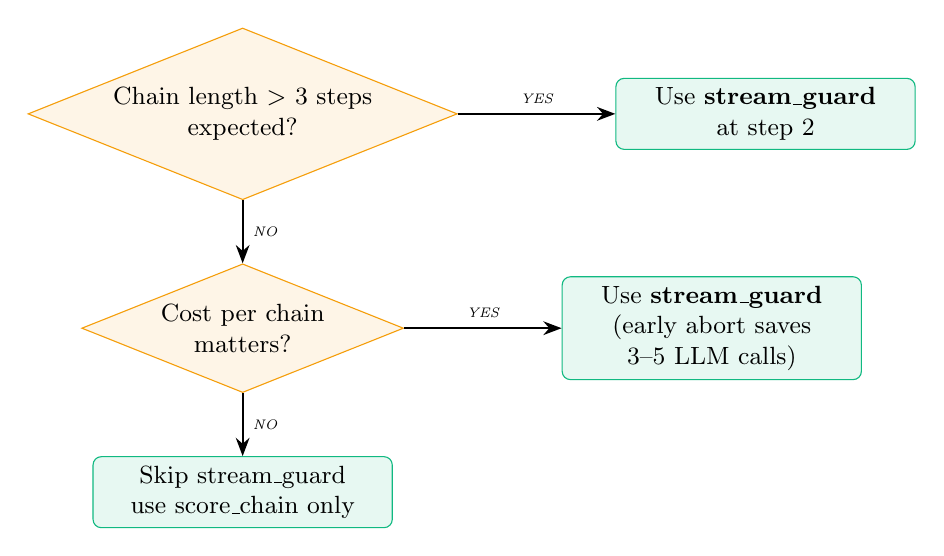
\begin{tikzpicture}[
  every node/.style={font=\small},
  decision/.style={diamond, draw=warning, fill=warning!10, aspect=2.5,
                   minimum width=4cm, align=center, inner sep=2pt},
  action/.style={rectangle, draw=success, fill=success!10,
                 rounded corners=3pt, minimum width=3.8cm,
                 minimum height=0.8cm, align=center},
  arr/.style={-{Stealth[length=5pt]}, thick},
  label/.style={font=\tiny\itshape, midway},
]
\node[decision] (D1) {Chain length $>$ 3 steps\\expected?};
\node[action, right=2cm of D1] (A1)
  {Use \textbf{stream\_guard}\\at step 2};
\node[decision, below=0.8cm of D1] (D2)
  {Cost per chain\\matters?};
\node[action, right=2cm of D2] (A2)
  {Use \textbf{stream\_guard}\\(early abort saves\\3--5 LLM calls)};
\node[action, below=0.8cm of D2] (A3)
  {Skip stream\_guard\\use score\_chain only};

\draw[-{Stealth}, thick] (D1) -- node[above, font=\tiny\itshape]{YES} (A1);
\draw[-{Stealth}, thick] (D1) -- node[right, font=\tiny\itshape]{NO} (D2);
\draw[-{Stealth}, thick] (D2) -- node[above, font=\tiny\itshape]{YES} (A2);
\draw[-{Stealth}, thick] (D2) -- node[right, font=\tiny\itshape]{NO} (A3);
\end{tikzpicture}
\end{center}

% ─────────────────────────────────────────────────────────────────────────────
\section{Performance Benchmarks}
% ─────────────────────────────────────────────────────────────────────────────

All AUROC figures are from held-out evaluation sets; no in-sample figures are
reported. Confidence intervals are computed via bootstrap (1000 resamples).

\begin{table}[h]
\centering
\small
\begin{tabular}{lllllr}
\toprule
\textbf{Method} & \textbf{Dataset} & \textbf{n} & \textbf{AUROC}
  & \textbf{95\% CI} & \textbf{Cost/chain} \\
\midrule
SC\_OLD behavioral & HotpotQA (within) & 200 & 0.817 & [0.74, 0.89] & \$0 \\
MiniJudge (LogReg+SC\_OLD) & HotpotQA 5-fold CV & 200 & $0.747\pm0.10$ & --- & \$0 \\
SC\_OLD & TriviaQA (cross) & 1000 & 0.659 & [0.614, 0.705] & \$0 \\
SC\_OLD & 2WikiMultiHop (cross) & 200 & 0.703 & [0.628, 0.775] & \$0 \\
SC\_OLD & NQ open-domain & 200 & 0.524 & [0.447, 0.609] & \$0 \\
+P(True) Haiku & TriviaQA & 37 & 0.720 & --- & $\sim$\$0.0003 \\
+P(True) blend $\alpha=0.25$ & TriviaQA & 37 & 0.737 & --- & $\sim$\$0.0003 \\
SC\_OLD+Sonnet (J5) & HotpotQA & 200 & 0.777 & --- & $\sim$\$0.007 \\
SC\_OLD+Sonnet (J5) & TriviaQA & 200 & 0.741 & --- & $\sim$\$0.007 \\
Alert precision @ 0.70 & HotpotQA & 200 & --- & P=0.908 & \$0 \\
CISC cost reduction & HotpotQA & 200 & identical & --- & $-41\%$ \\
\bottomrule
\end{tabular}
\caption{Full benchmark table. All results from held-out evaluation only.
NQ open-domain AUROC 0.524 reflects the harder factoid domain gap; behavioral
features are format-specific and degrade on truly unseen distributions.}
\end{table}

% ─────────────────────────────────────────────────────────────────────────────
\section{Integration Patterns}
% ─────────────────────────────────────────────────────────────────────────────

\subsection{Plain Python (simplest integration)}

\begin{lstlisting}
from llm_guard import AgentGuard

guard = AgentGuard()   # $0, no API key needed

# After your agent finishes
result = guard.score_chain(question, steps, final_answer)
if result.needs_alert:
    print(f"WARNING: risk={result.risk_score:.3f}, "
          f"mode={result.failure_mode}")
\end{lstlisting}

\subsection{Langfuse (trace + score)}

\begin{lstlisting}
from langfuse import Langfuse
from llm_guard import AgentGuard

langfuse = Langfuse()
guard    = AgentGuard()

def run_and_score(question, run_agent):
    with langfuse.trace(name="agent_run") as trace:
        steps, final_answer = run_agent(question)
        result = guard.score_chain(question, steps, final_answer)
        trace.score(
            name="llm_guard_risk",
            value=result.risk_score,
            comment=f"tier={result.confidence_tier}, "
                    f"mode={result.failure_mode}",
        )
    return final_answer, result
\end{lstlisting}

\subsection{LangSmith (evaluator protocol)}

\begin{lstlisting}
from langsmith.evaluation import EvaluationResult
from llm_guard import AgentGuard

guard = AgentGuard()

def llm_guard_evaluator(run, example):
    question     = example.inputs["question"]
    steps        = run.outputs.get("steps", [])
    final_answer = run.outputs.get("final_answer", "")
    result       = guard.score_chain(question, steps, final_answer)
    return EvaluationResult(
        key="llm_guard_risk",
        score=1.0 - result.risk_score,   # higher = better
        comment=f"tier={result.confidence_tier}",
    )

# Then: client.evaluate(dataset_name, evaluators=[llm_guard_evaluator])
\end{lstlisting}

\subsection{Prometheus (metrics + Grafana)}

\begin{lstlisting}
from prometheus_client import Histogram, Counter, start_http_server
from llm_guard import AgentGuard

RISK_HIST  = Histogram("llm_guard_risk_score", "Risk score distribution",
                        buckets=[0.1,0.2,0.3,0.4,0.5,0.6,0.7,0.8,0.9,1.0])
ALERT_CTR  = Counter("llm_guard_alerts_total", "Number of alert-level chains")

guard = AgentGuard(on_alert=lambda r: ALERT_CTR.inc())

def score_and_observe(question, steps, final_answer):
    result = guard.score_chain(question, steps, final_answer)
    RISK_HIST.observe(result.risk_score)
    return result

start_http_server(8000)   # Prometheus scrapes /metrics
\end{lstlisting}

\subsection{Datadog (DogStatsD)}

\begin{lstlisting}
from datadog import DogStatsd
from llm_guard import AgentGuard

statsd = DogStatsd()
guard  = AgentGuard()

def score_and_ship(question, steps, final_answer):
    result = guard.score_chain(question, steps, final_answer)
    statsd.gauge("llm_guard.risk_score", result.risk_score,
                 tags=[f"tier:{result.confidence_tier}",
                       f"mode:{result.failure_mode or 'none'}"])
    if result.needs_alert:
        statsd.increment("llm_guard.alerts",
                         tags=[f"mode:{result.failure_mode or 'none'}"])
    return result
\end{lstlisting}

% ─────────────────────────────────────────────────────────────────────────────
\section{API Quick Reference}
% ─────────────────────────────────────────────────────────────────────────────

\subsection{Public Methods}

\begin{table}[h]
\centering\small
\begin{tabularx}{\textwidth}{lllX}
\toprule
\textbf{Class} & \textbf{Method} & \textbf{Parameters} & \textbf{Returns} \\
\midrule
\texttt{MiniJudge} & \texttt{score()} & question, steps, final\_answer & float [0,1] \\
\texttt{MiniJudge} & \texttt{score\_chain()} & question, steps, final\_answer & float [0,1] \\
\texttt{MiniJudge} & \texttt{fit()} & chains, n\_splits=5 & MiniJudge \\
\texttt{AgentGuard} & \texttt{score\_chain()} & question, steps, final\_answer & ChainTrustResult \\
\texttt{AgentGuard} & \texttt{score\_with\_ptrue()} & question, steps, final\_answer & ChainTrustResult \\
\texttt{AgentGuard} & \texttt{generate\_trust\_object()} & question, steps, final\_answer & A2ATrustObject \\
\texttt{AgentGuard} & \texttt{stream\_guard()} & question, steps\_so\_far, abort\_threshold & StreamGuardResult \\
\texttt{AgentGuard} & \texttt{activate\_adapter()} & failure\_mode & AdapterResult \\
\texttt{AgentGuard} & \texttt{route\_to\_mesh()} & question, trust, agent\_answers & MeshResult \\
\texttt{AgentGuard} & \texttt{calibrate\_isotonic()} & scores, labels & AgentGuard \\
\texttt{A2ATrustObject} & \texttt{sign()} & secret & A2ATrustObject \\
\texttt{A2ATrustObject} & \texttt{verify()} & secret & bool \\
\texttt{A2ATrustObject} & \texttt{to\_dict()} & --- & Dict \\
\texttt{QuickCalibrator} & \texttt{fit()} & chains, domain & QuickCalibrator \\
\texttt{QuickCalibrator} & \texttt{score()} & question, steps, final\_answer & float \\
\texttt{probe\_ensemble\_blend()} & (module fn) & probe\_score, ptrue\_score, alpha=0.25 & float \\
\bottomrule
\end{tabularx}
\caption{All public API methods. \texttt{steps} is always a list of ReAct
step dicts with keys: \texttt{thought}, \texttt{action\_type},
\texttt{action\_args}, \texttt{observation}.}
\end{table}

\subsection{ChainTrustResult Fields}

\begin{table}[h]
\centering\small
\begin{tabularx}{\textwidth}{llX}
\toprule
\textbf{Field} & \textbf{Type} & \textbf{Description} \\
\midrule
\texttt{risk\_score} & float [0,1] & Composite risk (higher = more likely wrong) \\
\texttt{confidence\_tier} & str & \texttt{"HIGH"} / \texttt{"MEDIUM"} / \texttt{"LOW"} \\
\texttt{needs\_alert} & bool & True when risk\_score $\geq$ alert\_threshold (0.70) \\
\texttt{failure\_mode} & str|None & \texttt{"retrieval\_fail"} / \texttt{"repeated\_query"} /
  \texttt{"long\_chain"} / \texttt{"empty\_answer"} / None \\
\texttt{judge\_label} & str|None & \texttt{"GOOD"} / \texttt{"BORDERLINE"} / \texttt{"POOR"}
  (requires \texttt{api\_key} + \texttt{use\_judge=True}) \\
\texttt{behavioral\_score} & float & SC\_OLD score alone \\
\texttt{behavioral\_components} & Dict & Individual SC\_OLD feature scores (sc1--sc12) \\
\texttt{latency\_ms} & float & Scoring latency in milliseconds \\
\texttt{step\_count} & int & Number of Search steps in the chain \\
\bottomrule
\end{tabularx}
\caption{Fields of \texttt{ChainTrustResult} returned by \texttt{score\_chain()}.}
\end{table}

% ─────────────────────────────────────────────────────────────────────────────
\section{Telemetry Flywheel}
% ─────────────────────────────────────────────────────────────────────────────

\subsection{Architecture}

The telemetry flywheel allows users to contribute anonymised labels that
improve the shared MiniJudge model over time.

\begin{center}
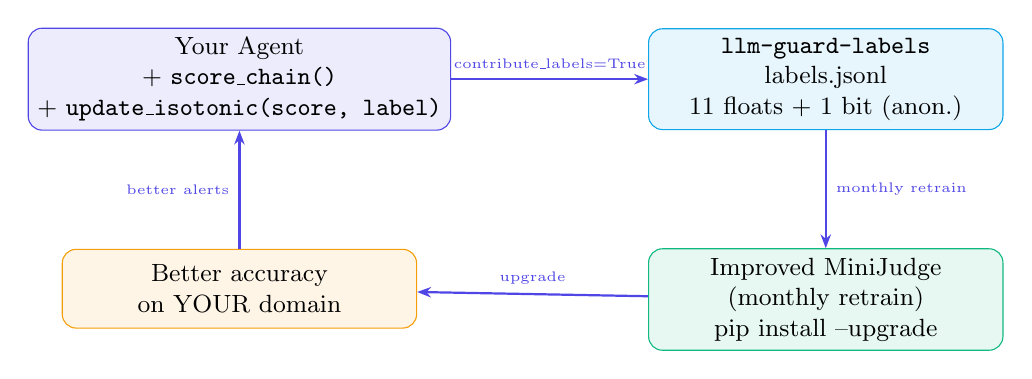
\begin{tikzpicture}[
  every node/.style={font=\small},
  box/.style={rectangle, rounded corners=5pt, draw, minimum width=4.5cm,
              minimum height=1cm, align=center},
  arr/.style={-{Stealth[length=5pt]}, thick, primary},
]

\node[box, fill=primary!10, draw=primary] (A)
  {Your Agent\\+ \texttt{score\_chain()}\\+ \texttt{update\_isotonic(score, label)}};

\node[box, fill=secondary!10, draw=secondary, right=2.5cm of A] (B)
  {\texttt{llm-guard-labels}\\labels.jsonl\\11 floats + 1 bit (anon.)};

\node[box, fill=success!10, draw=success, below=1.5cm of B] (C)
  {Improved MiniJudge\\(monthly retrain)\\pip install --upgrade};

\node[box, fill=warning!10, draw=warning, below=1.5cm of A] (D)
  {Better accuracy\\on YOUR domain};

\draw[arr] (A) -- node[above, font=\tiny]{contribute\_labels=True} (B);
\draw[arr] (B) -- node[right, font=\tiny]{monthly retrain} (C);
\draw[arr] (C) -- node[above, font=\tiny]{upgrade} (D);
\draw[arr] (D) -- node[left, font=\tiny]{better alerts} (A);

\end{tikzpicture}
\end{center}

\subsection{Privacy Guarantee}

Only the following data is transmitted when \texttt{contribute\_labels=True}:

\begin{itemize}
  \item \textbf{11 float features} (SC\_OLD structural scores: loop rate,
        empty-observation rate, step count, etc.)
  \item \textbf{1 correctness bit} (0 = correct, 1 = wrong)
\end{itemize}

\textbf{No question text, no answer text, no user data, no PII} is
transmitted. The 11 features are computed locally and contain no
recoverable content. Label contribution is \textbf{opt-in only} and
disabled by default.

\begin{lstlisting}
from llm_guard import AgentGuard

guard = AgentGuard()
result = guard.score_chain(question, steps, final_answer)

# After you know the ground truth:
guard.update_isotonic(result.behavioral_score, label=1)
# label=0 means correct, label=1 means wrong

# Opt-in to anonymised label contribution (default: False)
guard.contribute_label(result, correct=False,
                        github_pat=None)   # set PAT to contribute
\end{lstlisting}

% ─────────────────────────────────────────────────────────────────────────────
\section*{Quick Start}
% ─────────────────────────────────────────────────────────────────────────────

\begin{lstlisting}
pip install llm-guard-kit

from llm_guard import AgentGuard

guard = AgentGuard()   # zero cost, no API key

# Score a completed agent chain
result = guard.score_chain(
    question     = "What year was the Eiffel Tower built?",
    steps        = [
        {"thought": "Searching...", "action_type": "Search",
         "action_args": "Eiffel Tower year",
         "observation": "Built 1887-1889, completed for 1889 World Fair."},
        {"thought": "Got it.", "action_type": "Finish",
         "action_args": "1889", "observation": ""},
    ],
    final_answer = "1889",
)

print(f"Risk: {result.risk_score:.3f}  Tier: {result.confidence_tier}")
# >> Risk: 0.133  Tier: HIGH

if result.needs_alert:
    print("ALERT: possible wrong answer")
\end{lstlisting}

\vspace{1em}

\begin{center}
\small
\textbf{PyPI:} \url{https://pypi.org/project/llm-guard-kit/}
\quad\textbullet\quad
\textbf{GitHub:} \url{https://github.com/Avighan/llm-guard-kit}
\end{center}

\end{document}
